% =============================================================================
% AMR-Vortrag: Kolloquium / Verteidigung
% Fokus: Methodik, VDI 2206, Eigenschaftsabsicherung, Projektfragen
% Build: make vortrag_kolloquium.pdf
% =============================================================================
\documentclass[aspectratio=169]{beamer}
\usetheme{metropolis}

% Zentrales Design und alle Pakete laden
\usepackage{amr-style}

% -- Metadaten ---------------------------------------------------------------
\title{Autonomer mobiler Roboter fuer die Intralogistik}
\subtitle{Konzeption und Eigenschaftsabsicherung gemaess VDI 2206}
\author{Jan Unger}
\date{24. Maerz 2026}

% =============================================================================
\begin{document}
% =============================================================================

\maketitle

\begin{frame}{Gliederung}
  \small
  \tableofcontents
\end{frame}

% =============================================================================
\section{Motivation und Methodik}
% =============================================================================

\begin{frame}{Motivation und Problemstellung}
  \textbf{Ausgangslage und Problemstellung}
  \begin{itemize}
    \item Industrie 4.0 erfordert flexible Materialfluesse (z.\,B. KLT-Transporte).
    \item Industrielle AMR sind fuer diese Aufgaben oft ueberdimensioniert (Kosten $> 25\,000\,\mathrm{EUR}$).
    \item Technischer Kernkonflikt: Strikte Trennung von harter Echtzeit (Motorregelung) und rechenintensiver Navigation auf Low-Cost-Hardware.
  \end{itemize}

  \vspace{1em}
  \textbf{Methodik}\\
  Strukturierte Systementwicklung und Eigenschaftsabsicherung nach VDI 2206.
\end{frame}

\begin{frame}{Projektfragen (PF)}
  \begin{itemize}
    \item \textbf{PF1 -- Echtzeitarchitektur:}\\ Wie laesst sich auf einer Dual-Knoten-Architektur mit ESP32-S3 eine deterministische Regelung bei gleichzeitiger Sensorerfassung realisieren?
    \item \textbf{PF2 -- Navigationsgenauigkeit:}\\ Welchen Einfluss haben Odometrie-Kalibrierung, IMU-Fusion und hardwarenahe Sicherheitslogik auf die metrische Genauigkeit?
    \item \textbf{PF3 -- Wahrnehmung und Docking:}\\ Erreicht hybride Vision (Edge-Inferenz und Cloud-Semantik) eine ausreichend praezise Umgebungswahrnehmung fuer komplexe Innenraeume und zentimetergenaues Docking?
  \end{itemize}
\end{frame}

\begin{frame}{Methodisches Vorgehen: VDI 2206}
  \textbf{Entwicklung nach dem V-Modell}
  \begin{itemize}
    \item \textbf{Domaenenspezifischer Entwurf:} Aufteilung in Fahrkern (Phase 1), Sensorbasis (Phase 2) und Softwaredomaene (Phasen 3-4).
    \item \textbf{Iterative Zyklen:} Die Softwareentwicklung erforderte mehrfache Rueckspruege ueber die Arme des V-Modells.
    \item \textbf{Beispiel UMBmark:} Die Kalibrierung in der Eigenschaftsabsicherung (Phase 2) erzwang eine Korrektur der Parameter in \texttt{config\_drive.h} und damit einen Ruecksprung in den Entwurf.
  \end{itemize}
\end{frame}

% =============================================================================
\section{Systemarchitektur und Hardware}
% =============================================================================

\begin{frame}{Architektur der Drei Ebenen}
  \begin{figure}[htbp]
    \centering
    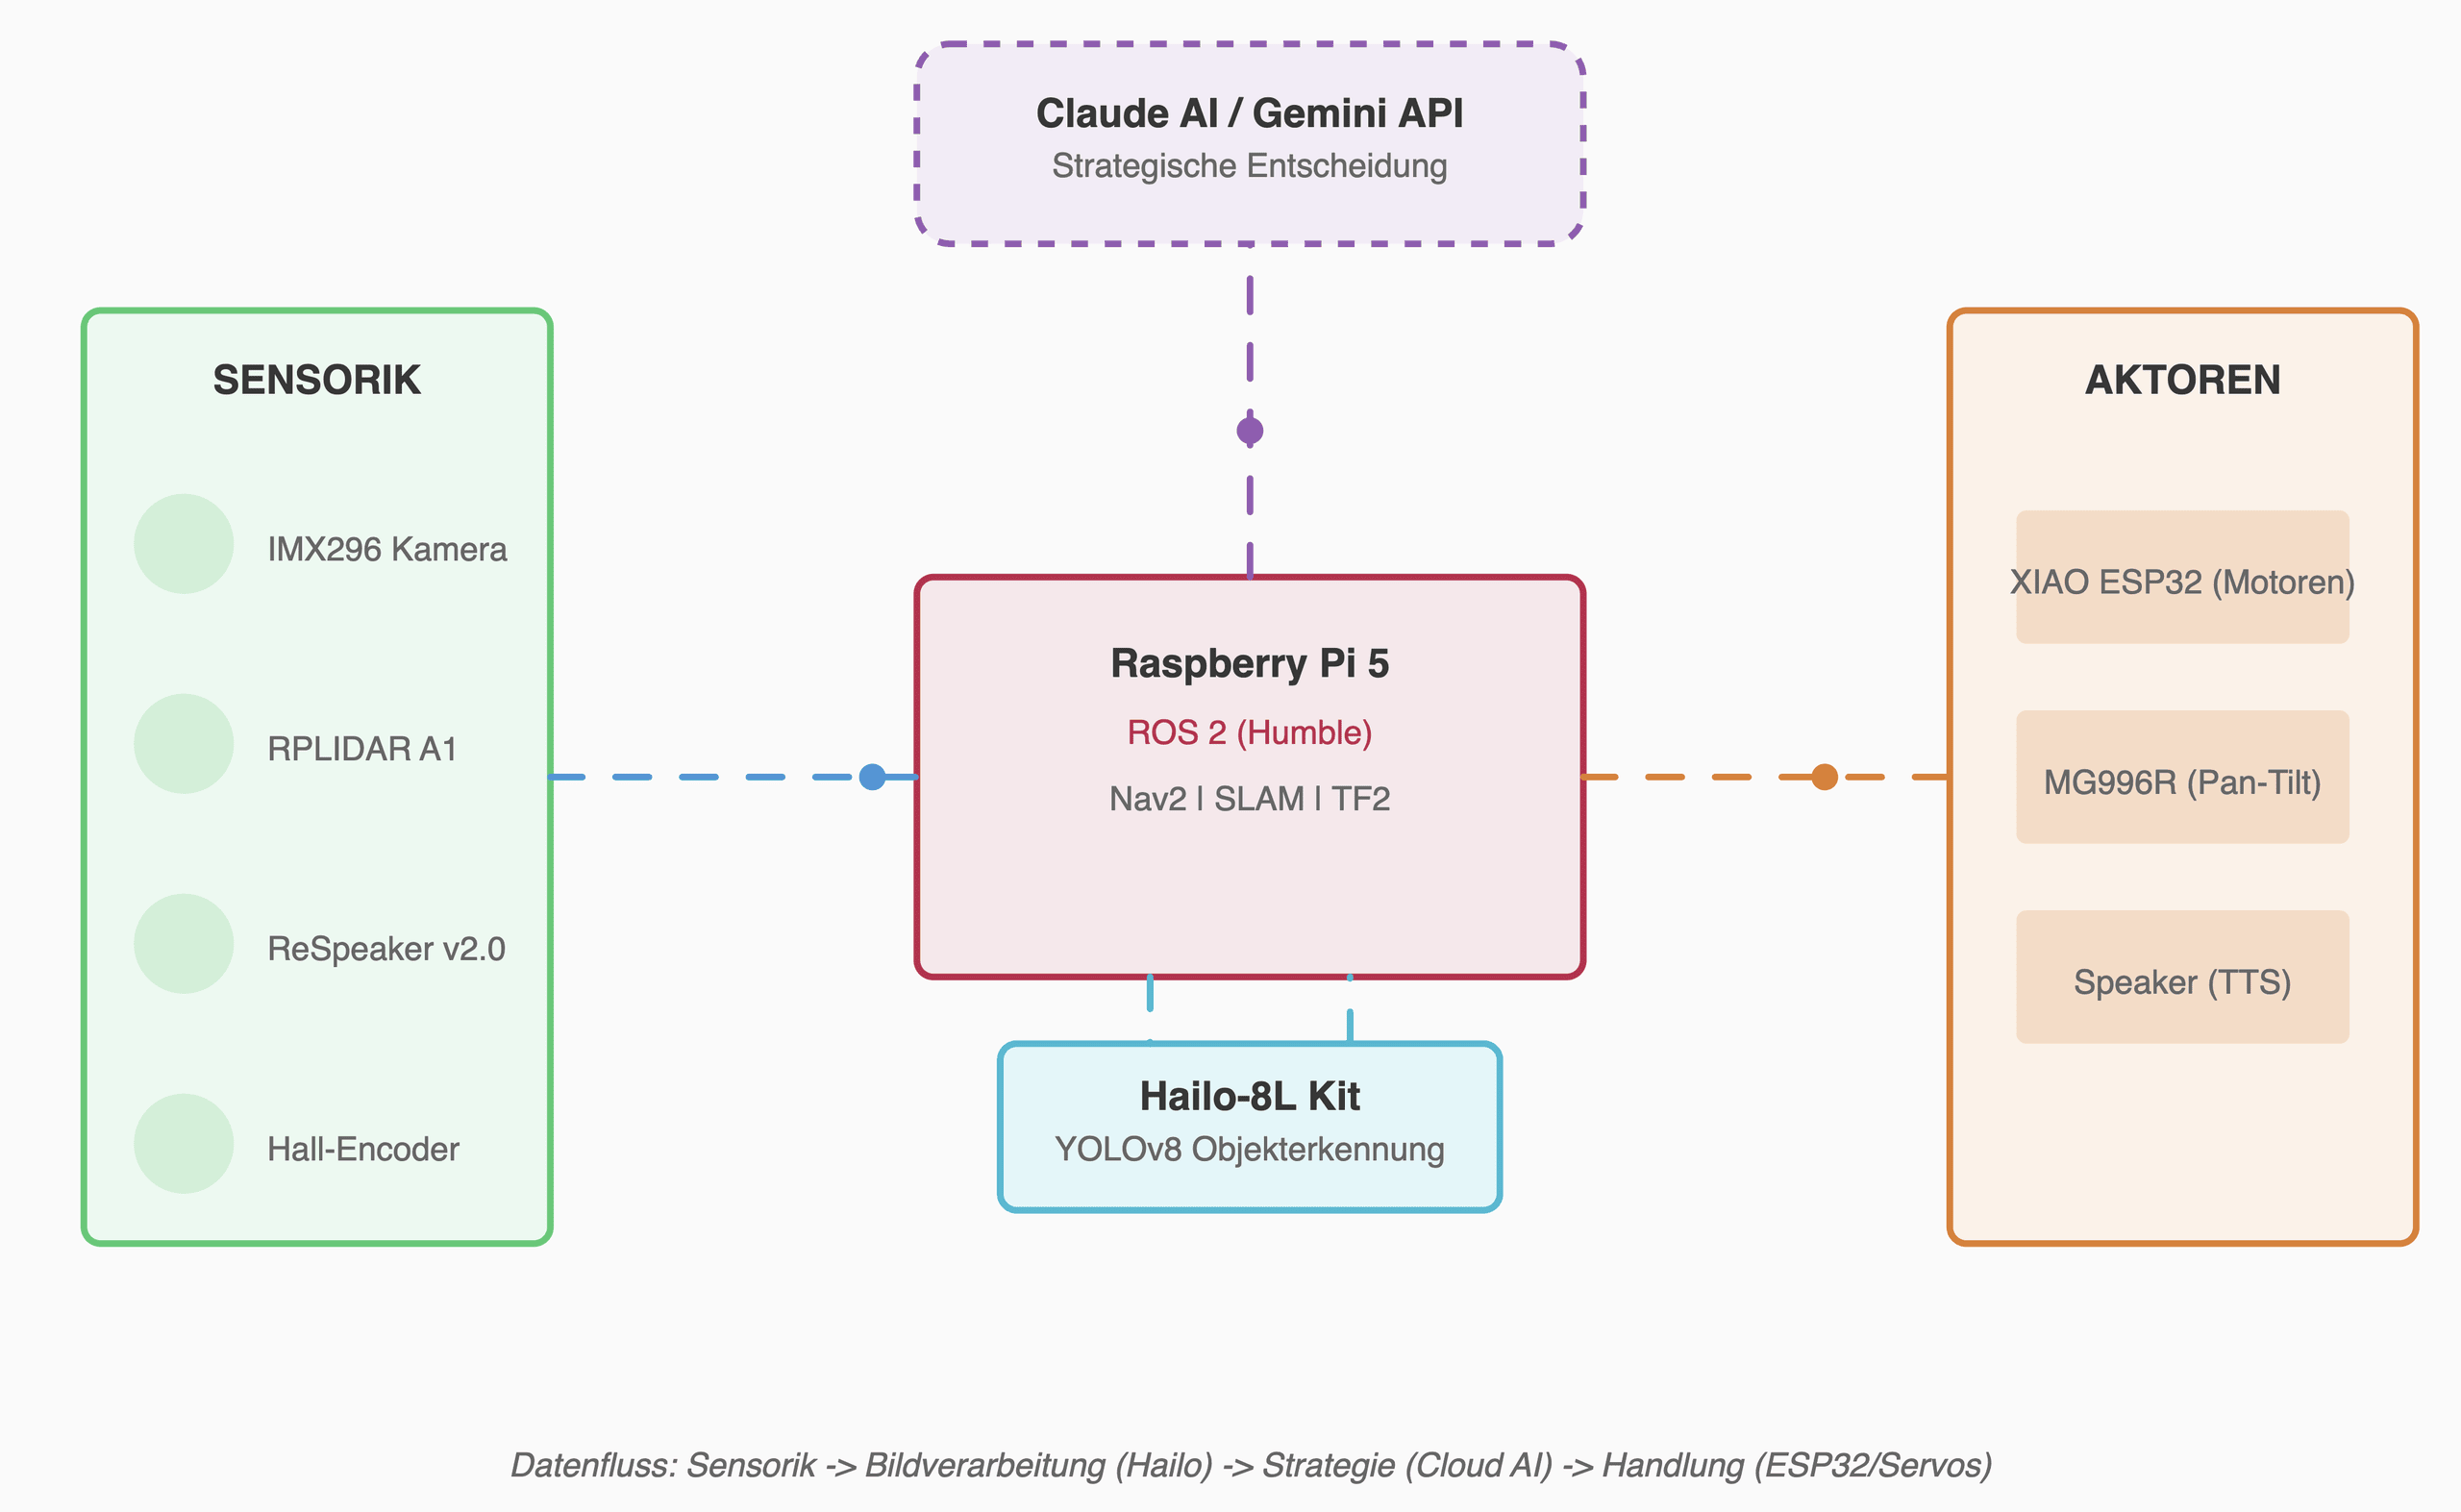
\includegraphics[width=0.45\textwidth]{amr_datenfluss.pdf}
  \end{figure}
  \vspace{-1em}
  \begin{itemize}
    \item \textbf{Fahrkern und Sensorbasis (Ebene A):} Zwei ESP32-S3 steuern deterministisch Antrieb und Sensorik. CAN-Notstopp funktioniert ohne Pi~5.
    \item \textbf{Bedien- und Leitstandsebene (Ebene B):} RPi~5 mit ROS2, Nav2, SLAM; Benutzeroberflaeche (React/Zustand, WSS:9090, MJPEG:8082).
    \item \textbf{Intelligente Interaktion (Ebene C):} Hailo-8L Edge-NPU, Gemini Cloud-Semantik, Sprachsteuerung (ReSpeaker + Gemini STT), TTS.
  \end{itemize}
\end{frame}

\begin{frame}{Aktorik: Der Dual-Core Mikrocontroller}
  \textbf{Ressourcentrennung auf dem Drive-Knoten (ESP32-S3)}
  \begin{itemize}
    \item \textbf{Core 0 (Kommunikation):} Betreibt den micro-ROS-Executor und ueberwacht den Heartbeat von Core 1.
    \item \textbf{Core 1 (Regelung):} Fuehrt exklusiv die PID-Regelschleife mit $50\,\mathrm{Hz}$ aus.
    \item \textbf{Inverskinematik:} Berechnet individuelle Sollradgeschwindigkeiten basierend auf \texttt{cmd\_vel}-Vorgaben.
    \item \textbf{Vorteil:} Vermeidung von Jitter durch blockierende I2C-Sensorabfragen.
  \end{itemize}
\end{frame}

\begin{frame}{Hardwarenahe Sicherheitslogik}
  \textbf{Zwei unabhaengige Sicherheitspfade}
  \begin{itemize}
    \item \textbf{ROS-2-Pfad (Multiplexer):} Der \texttt{cliff\_safety\_node} blockiert Navigationsbefehle bei erkannter Kante. Callback-Latenz (\texttt{cliff\_safety\_node}): $2{,}0\,\mathrm{ms}$.
    \item \textbf{CAN-Notstopp-Redundanz:} Ein hardwarenaher CAN-Bus uebertraegt Cliff-Signale (CAN-ID 0x120) direkt zwischen den Mikrocontrollern.
    \item \textbf{Reaktionszeit:} $< 20\,\mathrm{ms}$ CAN-zu-Motor-Reaktion (Drive-Node), Gesamtkette Cliff-Erkennung $\rightarrow$ Motor-Stopp ca.\ $73\,\mathrm{ms}$.
  \end{itemize}
\end{frame}

\begin{frame}{Bedien- und Leitstandsebene (Dashboard)}
  \textbf{Webbasierte Benutzeroberflaeche (Ebene B)}
  \begin{itemize}
    \item \textbf{Tech-Stack:} React 19, TypeScript, Zustand Store ($60+$ Telemetrie-Properties), Tailwind CSS.
    \item \textbf{Vier Seiten:} Steuerung (Joystick, Karte, Kamera), Details (Sensoren, System), Validierung (15 Tests), Sprache.
    \item \textbf{Kommunikation:} WebSocket (WSS:9090, auto-reconnect) und MJPEG-Kamerastream (:8082). Rate-Limiting: Joystick $10\,\mathrm{Hz}$, Heartbeat $5\,\mathrm{Hz}$, Servo $10\,\mathrm{Hz}$.
    \item \textbf{Totmannschalter:} $300\,\mathrm{ms}$ Deadman-Timer --- bei Verbindungsverlust automatischer Notstopp (\texttt{cmd\_vel} $= 0$).
  \end{itemize}
\end{frame}

% =============================================================================
\section{Lokalisierung, Navigation und Vision}
% =============================================================================

\begin{frame}{Lokalisierung: Der TF-Baum}
  \begin{figure}[htbp]
    \centering
    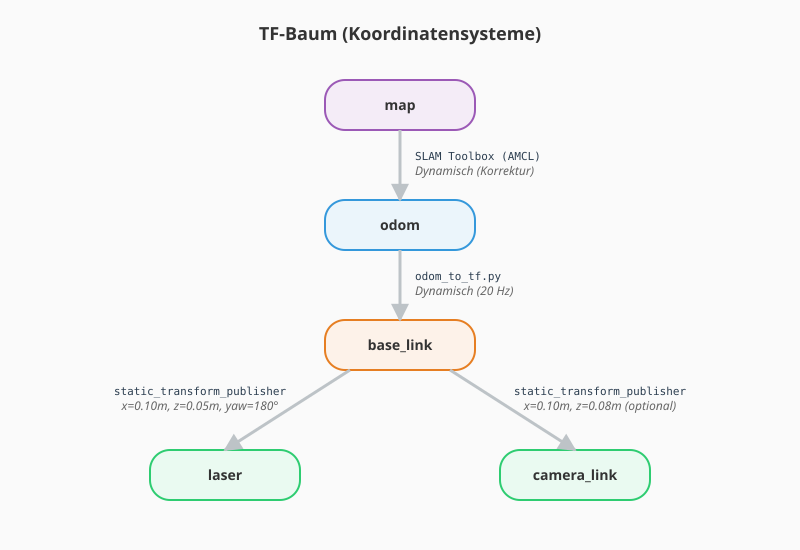
\includegraphics[height=0.45\textheight]{amr_tf_baum.pdf}
  \end{figure}

  \vspace{0.5em}
  \textbf{Koordinatensysteme (REP-105)}
  \begin{itemize}
    \item \texttt{map $\rightarrow$ odom}: Drift-Korrektur durch SLAM Toolbox und AMCL.
    \item \texttt{odom $\rightarrow$ base\_link}: Berechnet aus Rad-Odometrie ($20\,\mathrm{Hz}$).
    \item \texttt{base\_link $\rightarrow$ laser}: Statische Extrinsik ($x = 0{,}10\,\mathrm{m}$, Yaw = $180^\circ$).
  \end{itemize}
\end{frame}

\begin{frame}{Hybride Vision-Pipeline}
  \textbf{Edge-Inferenz und Cloud-Semantik (Ebene C)}
  \begin{itemize}
    \item \textbf{Edge-KI:} Hailo-8L NPU ($1{,}5\,\mathrm{W}$ typ.) fuehrt YOLOv8-Objekterkennung mit $5\,\mathrm{Hz}$ Pipeline-Rate aus (ca.\ $34\,\mathrm{ms}$ Inferenzzeit). UDP-Bruecke Host $\rightarrow$ Docker.
    \item \textbf{Cloud-Semantik:} \texttt{gemini\_semantic\_node} (Modell: \texttt{gemini-3.1-flash-lite}) sendet Detektionen und Telemetrie an Gemini API fuer kontextbasierte Situationsbewertung.
    \item \textbf{Sprachausgabe (TTS):} gTTS Cloud-Synthese $\rightarrow$ mpg123 $\rightarrow$ MAX98357A I2S-Lautsprecher. Gemini-Semantik wird gesprochen (Rate-Limit: $10\,\mathrm{s}$).
    \item \textbf{Vorteil:} Die rechenintensive Wahrnehmung gefaehrdet die Echtzeitfaehigkeit des Nav2-Stacks nicht.
  \end{itemize}
\end{frame}

\begin{frame}{Sprachsteuerung (Ebene C)}
  \textbf{Natuerlichsprachliche Interaktion via Gemini STT}
  \begin{itemize}
    \item \textbf{Pipeline:} ReSpeaker-Mikrofon (VAD) $\rightarrow$ Audioaufnahme $\rightarrow$ Gemini Flash STT + Intent-Erkennung in einem API-Call $\rightarrow$ Befehlsausfuehrung.
    \item \textbf{State-Machine:} IDLE $\rightarrow$ LISTENING $\rightarrow$ PROCESSING $\rightarrow$ COOLDOWN. Barge-In-Schutz ($2\,\mathrm{s}$).
    \item \textbf{Befehle:} Fahren, Drehen, Stopp, LED-Steuerung, Servo, ``Dreh dich zu mir'' (DoA-Quadranten), Standort, Wetter.
    \item \textbf{Dashboard-Integration:} VoicePage mit Live-Transkription, Mikrofon-Mute und Kommandoverlauf.
  \end{itemize}
\end{frame}

% =============================================================================
\section{Eigenschaftsabsicherung und Ergebnisse}
% =============================================================================

\begin{frame}{Eigenschaftsabsicherung (PF1 und PF2)}
  \textbf{Verifikation der hardwarenahen Subsysteme}

  \vspace{0.2em}
  {\small
  \begin{tabular}{@{}lll@{}}
    \toprule
    \textbf{Metrik} & \textbf{Messergebnis} & \textbf{Akzeptanzkriterium} \\
    \midrule
    PID-Regelfrequenz    & $50\,\mathrm{Hz}$ (Jitter $< 2\,\mathrm{ms}$) & erfuellt \\
    Callback-Latenz (\texttt{cliff\_safety\_node}) & $2{,}0\,\mathrm{ms}$ & $< 50\,\mathrm{ms}$ \\
    Geradeausfahrt-Drift & $2{,}1\,\mathrm{cm}$ (mit IMU-Fusion) & $< 5{,}0\,\mathrm{cm}$ \\
    \bottomrule
  \end{tabular}}

  \vspace{0.8em}
  \textbf{Validierung der Systemnavigation und des Dockings (PF2 und PF3)}

  \vspace{0.2em}
  {\small
  \begin{tabular}{@{}lll@{}}
    \toprule
    \textbf{Metrik} & \textbf{Messergebnis} & \textbf{Akzeptanzkriterium} \\
    \midrule
    ATE RMSE (Kartierung) & $0{,}19\,\mathrm{m}$ & $< 0{,}20\,\mathrm{m}$ \\
    Positionsgenauigkeit (Nav2) & $1{,}01\,\mathrm{cm}$ (max.\ $2{,}17\,\mathrm{cm}$) & $< 10\,\mathrm{cm}$ \\
    ArUco-Docking (10/10) & $0{,}73\,\mathrm{cm}$ mittl.\ Versatz & $< 5\,\mathrm{cm}$ \\
    Docking-Orientierung & $14{,}1^\circ$ mittl.\ Abweichung & --- \\
    \bottomrule
  \end{tabular}}
\end{frame}

% =============================================================================
\section{Zusammenfassung}
% =============================================================================

\begin{frame}{Fazit und Projektbeantwortung}
  \textbf{Kernergebnisse}
  \begin{itemize}
    \item \textbf{PF1 (Bestaetigt):} Die Dual-Knoten-Architektur stabilisiert die Echtzeit. Die UART-Kopplung ($921\,600\,\mathrm{Baud}$) loest Latenzprobleme drahtloser Systeme.
    \item \textbf{PF2 (Bestaetigt):} UMBmark-Kalibrierung; Geradeausfahrt-Drift von $3{,}6$ auf $2{,}1\,\mathrm{cm}$ durch IMU-Fusion. Nav2-Waypoint-Praezision: $1{,}01\,\mathrm{cm}$ mittlerer Fehler.
    \item \textbf{PF3 (Bestaetigt):} ArUco-Docking $100\,\%$ (10/10, Dreifach-Bedingung bei $0{,}30\,\mathrm{m}$, $0{,}73\,\mathrm{cm}$ mittlerer Versatz). Grenzen bei unzureichender Beleuchtung.
  \end{itemize}

  \vspace{0.8em}
  \textbf{Fazit:}\\
  Ein kostenguenstiges Gesamtsystem (${\sim}\,694\,\mathrm{EUR}$) erfuellt intralogistische Grundlagenanforderungen gemaess VDI 2206. Alle fuenf Validierungsphasen bestanden (Phasen 1--5 PASS). Die Grenzen liegen in den MTU-Beschraenkungen ($512$ Bytes) und Rad-Schlupf.
\end{frame}

\end{document}
